\section{Related Work}\label{sec:relatedwork}

In this section, we compare ML4PG with tools available in Coq and other ITPs, an overview of this comparison is provided in
Table~\ref{tab:comparison}.

\begin{table}
\tbl{\scriptsize{\emph{Comparison of ML4PG with premise-selection methods, Coq's search mechanisms and dependency graphs.}}\label{tab:comparison}}{
\centering
{\scriptsize
 \begin{tabular}{ p{2cm}  p{1.75cm}  p{1.75cm}  p{1.75cm}   p{1.75cm}   p{1.75cm} }
   \toprule
    & Premise Selection & Search & Dependency graphs & Model Inference & ML4PG  \\
		%\hline
		%\hline
  	%	Fib example & No & No &   \alert{Yes} \\
		%	\hline
\midrule
\midrule
\textbf{Method} & Statistical Proof-Premise Selection & Search & Parsing & Model Inference &  Statistical Pattern-recognition \\

\midrule
   \textbf{Goal-oriented?} & Yes  & Yes &  Not necessarily & No & Not necessarily  \\
\midrule
   \textbf{Deterministic?} & No & Yes &Yes  & No & No   \\
\midrule
	\textbf{Visual representation} & No & No  & Yes  & Yes   & Yes \\
\midrule
	\textbf{Covers proofs or terms?} & Both &Terms/types & Both & Proofs  &  Both  \\
\midrule	
			\textbf{Takes into consideration dependencies?} & Yes & No & Yes & Yes  & Yes \\
\midrule
		\textbf{Finds structural similarities beyond concrete syntax?} & No & No & No  & No & Yes  \\
\midrule
	\textbf{Finds structurally similar patterns in proofs?} & No & No & No & No  & Yes  \\
\midrule
  \textbf{Good for proof automation?} & Depend on background theory & No & No & Depend on background theory & Depend on background theory \\
   \bottomrule
		\end{tabular} }}
\end{table}


\paragraph{Statistical Proof-Premise Selection in ITPs} Proof automation in ITPs has been enhanced with the connection of this kind of 
systems with Automated Theorem Provers (ATPs). The workflow of tools like Sledgehammer~\cite{Paulson_threeyears} or HolyHammer~\cite{holyhammer} consists of the following steps: (1) translation of the statement of the theorem (from the ITP format) to a
first order format suitable for ATPs; (2) selection of the lemmas (or premises) that could be relevant to prove a theorem; 
(3) invocation of several ATPs to prove the result; and (4) if an ATP is successful in the proof, reconstruction of the proof in
the ITP from the output generated by the ATP.

An important issue in the above procedure is the premise selection mechanism, especially when dealing with big libraries, since proofs of some results can be infeasible for the ATPs if they receive too many premises. Statistical machine-learning methods have been 
successfully used to tackle this problem in~\cite{UrbanSPV08,K13,holyhammer}. In particular, a classifier is constructed for every 
lemma of the library. Given two lemmas $A$ and $B$, if $B$ was used in the proof of $A$, a feature vector $|A|$  is extracted 
from the statement of $A$, and is sent as a positive example to the classifier $<B>$ constructed for $B$; otherwise, $|A|$ is
used as a negative example to train $<B>$.
Note that, $|A|$  captures statistics of $A$'s syntactic form relative to
every symbol in the library; and the resulting feature vector is a sparse (including up to $10^6$ features).
 After such training, the classifier $<B>$ can predict whether a new lemma $C$ requires 
the lemma $B$ in its proof, by testing $<B>$ with the input vector $|C|$. On the basis of such predictions for all lemmas in the library,  this tool constructs a hierarchy of the premises that are most likely to be used in the proof
of $C$. 

There are several differences between the statistical premise-selection tools and ML4PG:

\begin{itemize}
 \item \emph{Aim:} premise selection tools help the prover, trying to increase the number of goals automatically proved by ATPs, and ML4PG
 assists the user, providing suggestions as proof hints.
 \item \emph{Features:} premise selection tools extract features from first-order formulas translated from the original syntax of the
 theorem prover; on the contrary, ML4PG directly works with Coq's higher-order formulas and proofs. 
 \item \emph{Dependencies:} premise selection tools capture the dependencies of lemmas used in the proof of theorems; ML4PG not only 
 captures these dependencies but also information about, for instance, tactics involved in a proof.
 \item \emph{Machine-learning methods:} Premise selection tools use supervised learning methods, and ML4PG uses unsupervised techniques.
 \item \emph{Proof Automation:} the success of tools like Sledgehammer depends on several aspects: good methods for premise selection,
 availability of a useful background theory, and success of ATPs and the proof reconstruction tool. In the case of ML4PG, the 
 availability of a background theory is also a key aspect for success proof automation, but it also depends on the existence of 
 theorems that required similar proofs. Hence, both tools are only as good as the background theory that was previously developed. \end{itemize}

% As in the case of proof-automation in ML4PG (cf. Section~\ref{sec:evaluation}), tools like Sledgehammer~\cite{Paulson_threeyears} or HolyHammer~\cite{holyhammer} are only as good as the background theory that was previously developed. Therefore, premise selection tools
% can improve the performance of those tools as long as the necessary lemmas are available.


\paragraph{ML4PG vs Coq's Searching Tools} Coq/SSReflect already provides comprehensive search mechanisms to inspect the corpus of results available in different libraries.
There are several search commands in Coq:  \lstinline?Search?~, \lstinline?SearchAbout?, \lstinline?SearchPattern?
and \lstinline?SearchRewrite?~\cite{Coq}. In addition, SSReflect implements its own version of the \lstinline?Search?
command \cite{SSReflect} --- SSReflect's \lstinline?Search? gathers the functionality of the 4 Coq's search commands.
The Whelp platform~\cite{AspertiGCTZ04} is a web search engine for mathematical knowledge formalised in Coq, which features 3 functionalities:
\lstinline?Match? (similar to Coq's \lstinline?Search? command), \lstinline?Hint? (that finds all the theorems which can
be applied to derive the current goal) and \lstinline?Elim? (that retrieves all the eliminators of a given type).
%In this section, we compare ML4PG with these tools.  

%Let us explain first when these tools are usually invoked. 
The existing search mechanisms can be used in two different scenarios. If the user knows how to continue the proof, but
he does not remember (or know) the concrete name of the desired auxiliary lemma, it suffices to provide a search pattern to Coq searching engines, e.g.
using commands of the form
``\lstinline?Search "distr"? \lstinline?in bigop?'' or   
``\lstinline?Search _ (_ * (\big[_/_]_(_ <- _| _) _))?'',
 where \texttt{bigop} is a library, \texttt{"distr"} is a pattern in a lemma name, and  \lstinline? _ (_ * (\big[_/_]_(_ <- _| _) _))?
is a pattern for search.
 
%\begin{example}\label{ex:distr}
% In the proof of Lemma~\ref{lem:nilpotent}, we may want to introduce the term $(1-M)$ inside the sum $\sum_{i=0}^{n-1} M^i$, but 
% if we have no experience with the bigop library of SSReflect, it is likely that we do not know the name of the concrete lemma. 
% The lemma which carries out this task can be find using, for instance, the commands \lstinline?Search "distr" in bigop.? or  
%\lstinline?Search _ (_ * (\big[_/_]_(_ <- _| _) _))?. 
%\end{example}
In the second scenario, the user needs help in the middle of the proof. Searching mechanisms can be also useful in this 
case; for instance, using the \lstinline?Search? command the user can search all the lemmas associated with a concrete term
of the current goal. The \lstinline?Hint? mechanism of Whelp can find all the theorems which can be applied to derive the current goal.

%\begin{example}\label{ex:fact}
% In the proof of Lemma~\ref{lem:factorial}, we can find all the lemmas related to the factorial function using the command
% \lstinline?SearchAbout factorial?. 
%\end{example}

%ML4PG is helpful in the second scenario, since it provides families of similar proofs. Inspecting that family of proofs, 
%the user can find a pattern to finish the proof that she is formalising. 

%As we have seen in Examples~\ref{ex:distr} and~\ref{ex:fact}, 
The above search mechanisms are goal directed and deterministic. That is, the user
searches  the chosen  libraries for lemmas related to a concrete type, term or pattern. 
If the patterns defined by the user are present in the given library, then the user is guaranteed to see the relevant lemmas on the screen.

The situation is more complicated if the user does not know the right pattern to search for. Imagine, for example, being in the middle of constructing a proof, 
and wishing to get some higher-level hint on how to proceed, wishing there was an ITP expert near, who would suggest a further proof strategy based on his previous experience. ML4PG was created to emulate such intelligent help automatically, using statistical machine-learning algorithms to use the information arising from the ``previous experience''.

In comparison to the more traditional \emph{search engines}, ML4PG is a goal-independent (unsupervised) tool, i.e. the user does not have to know the required pattern in advance. But, as many statistical machine-learning applications, it is also non-deterministic. That is, the tool failing to suggest a proof pattern does not mean there is no ``interesting'' pattern to be found. Actually, the notion of a proof pattern being ``interesting'' is left to the user's judgement, as well. 

\paragraph{ML4PG vs Coq's Visualisation Tools} Several visualisation tools have been developed to facilitate the understanding
of the dependencies that arise in Coq developments. Namely, Coq provides tools to visualise dependencies among files, dependencies 
between theorems and definitions, proof-trees, and proof-models.

Large Coq developments involve hundreds of files (e.g. 125 files in the proof of the Feit-Thompson theorem); therefore, the 
computation and visualisation of the dependencies among those files is an important issue to maintain those developments. The 
Coq distribution provides the \lstinline?coqdep? tool to compute file dependencies. The output generated by \lstinline?coqdep? 
can be fed into the tool developed in~\cite{dependtohtml} to visualise file dependencies (see Figure~\ref{fig:depend-files}). 

\begin{figure}[t]
\centering 
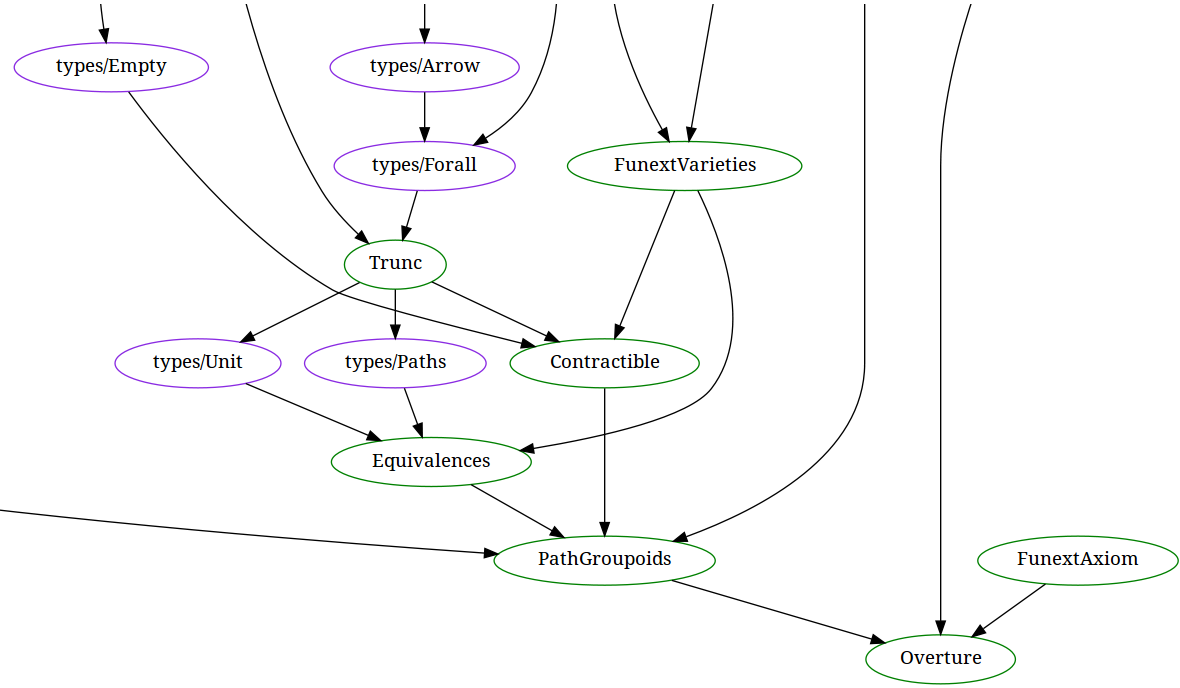
\includegraphics[scale=.4]{HoTTCorefragment.png}
\caption{\scriptsize{\emph{Fragment of the dependency graph of the HoTT library.} The complete dependency graph is available at the HoTT wiki\protect\cite{hottbook}.}}\label{fig:depend-files}
\end{figure}

A different set of tools~\cite{dpdgraph,BPP00} has been developed to compute and visualise dependencies between theorems and definitions, see Figure~\ref{fig:dgraph1}. An analysis of proof terms makes it possible to know whether some theorem is used when proving another result or when defining a new concept. Visualising the complete graph of dependence is useful to detect the results that are not used, and to foresee the impact of modifying a theorem or definition.  

These dependency graphs are designed to, mainly, work with proofs rather than object definitions and do not show the term structure per se,
but only the dependencies between the auxiliary lemmas/constructors used. Moreover, they give a complete information of all the results that were necessary to prove a given lemma, making hard to read them, due to the presence of this complete information. Hence,  statistical machine learning may be useful for data-mining the above information in order to discriminate unimportant features of the
lemma, and highlight those that are important. ML4PG essentially does this. ML4PG's recurrent clustering  captures term and lemma dependencies recurrently, via the feature extraction which itself involves recurrent clustering of all previously
defined terms. 


ML4PG's proof clustering in particular is very close to dependency graphs for lemmas, in that both are capturing mutual or inductive dependencies of all lemmas needed to prove the given statement. As a result, ML4PG can be seen as a post-processing tool for dependency
graphs. Given a big graph as shown in Figure~\ref{fig:dgraph1}, what is the right way to discriminate its unimportant features? How to decide which of them are important or not? One of the ways to do this, is to determine that relatively to other lemmas in the library. This is achieved by applying clustering in ML4PG. Taking all of the above features into account, ML4PG can associate various object definitions
and lemma statements and lemma proofs. 

\begin{figure}
\centering
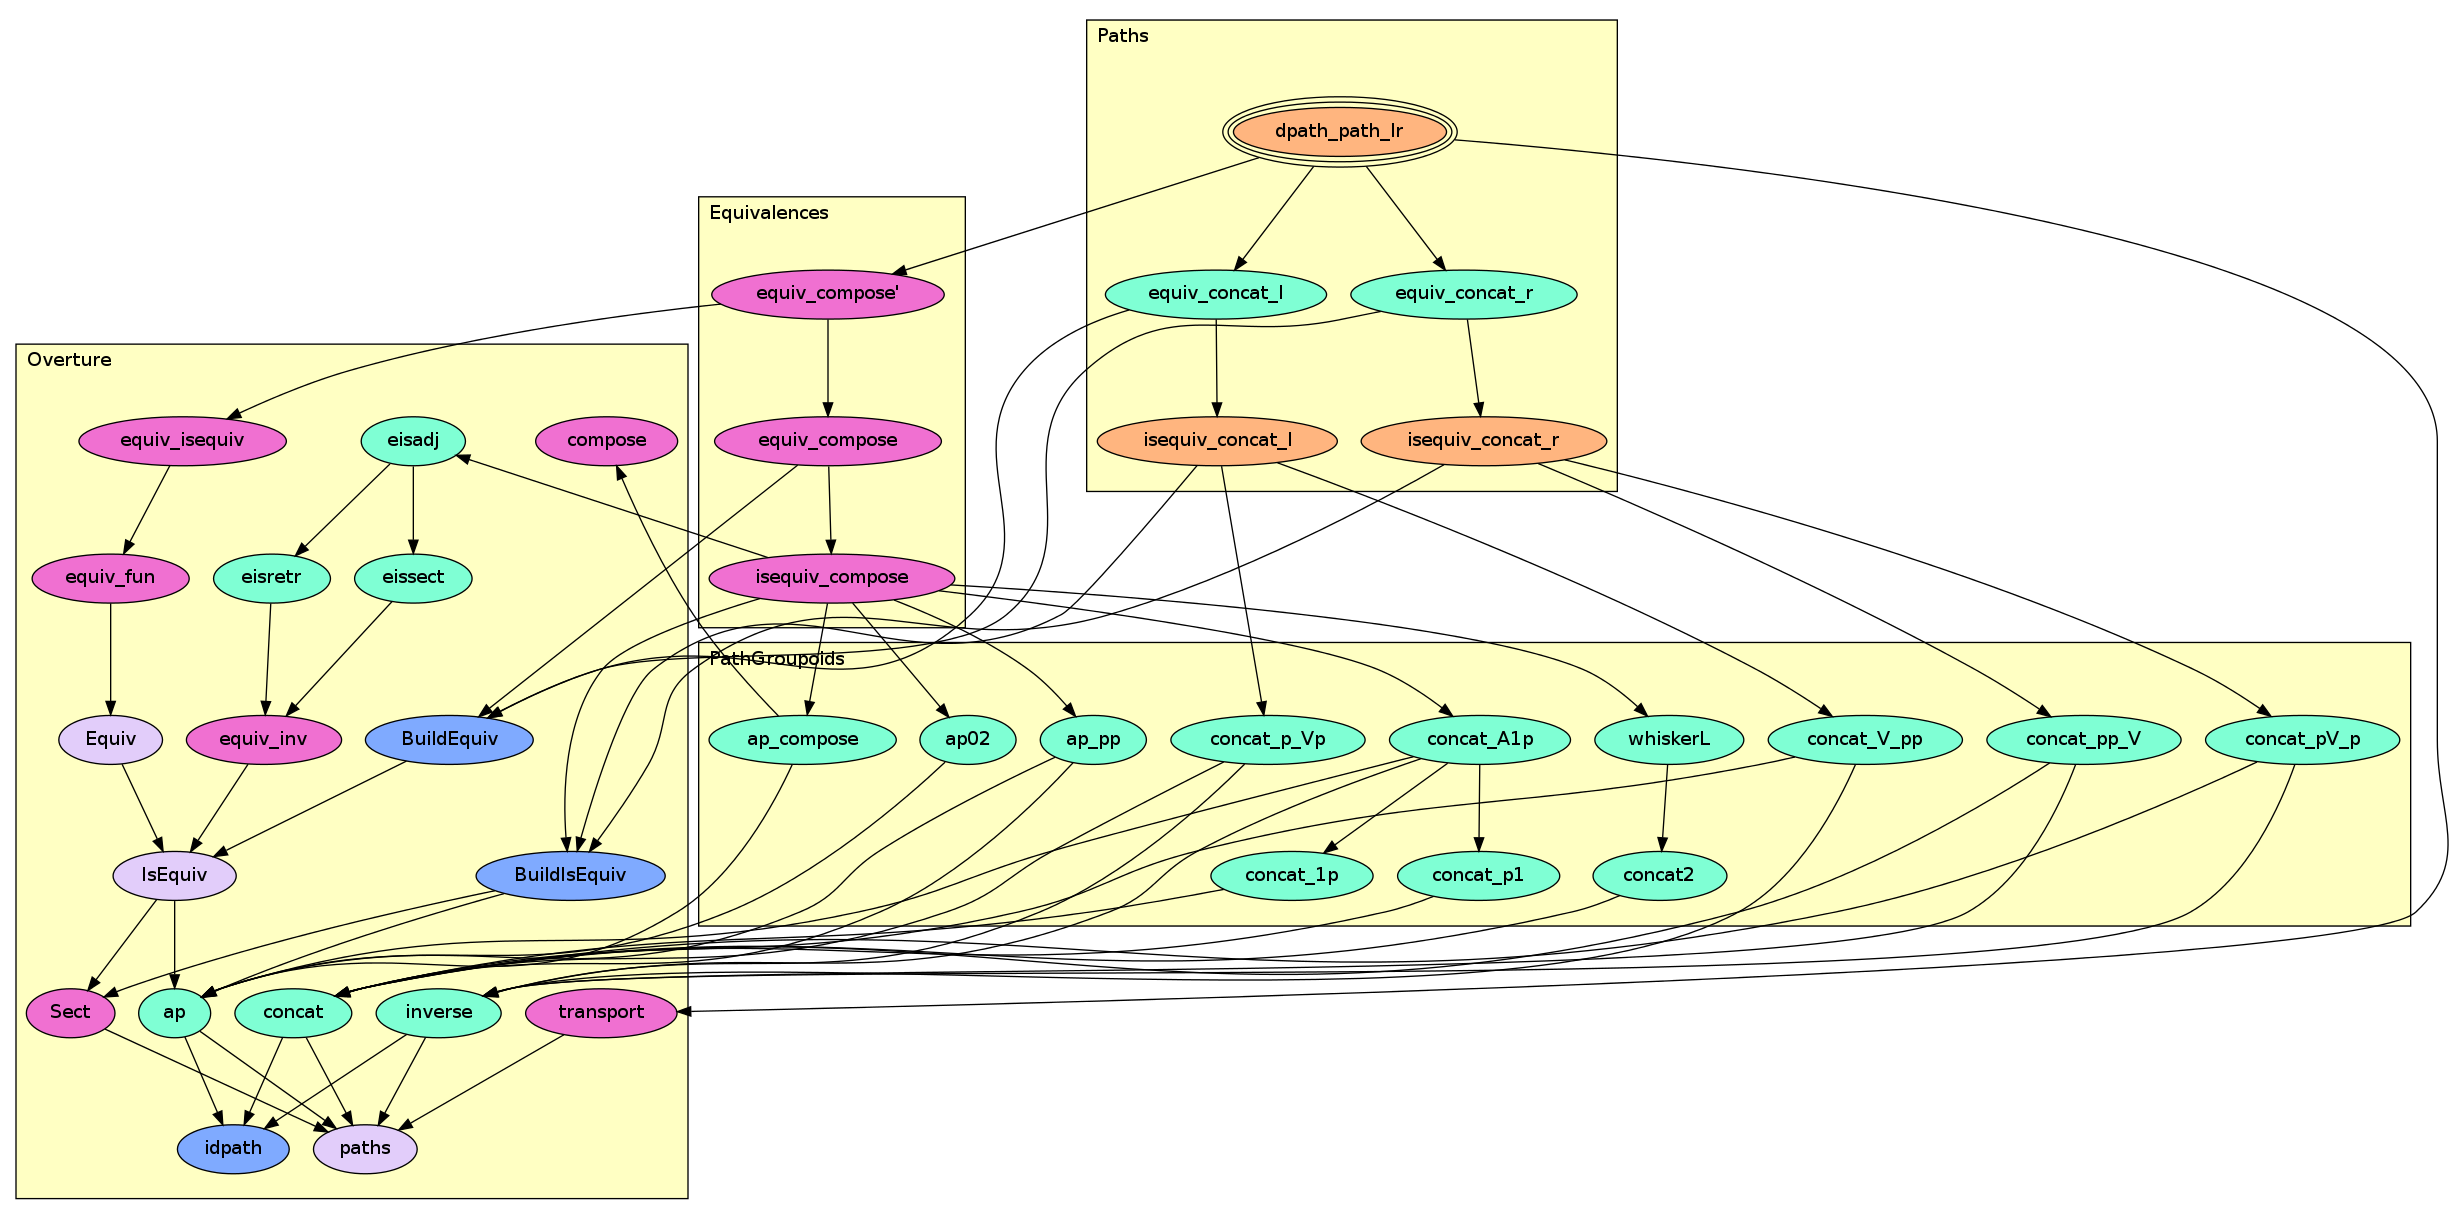
\includegraphics[scale=.15]{graph_dpath_path_lr.png}
\caption{\scriptsize{\emph{Dependency graph for the theorem \texttt{dpath\_path\_lr} included in the \texttt{Paths} library of HoTT.}}}\label{fig:dgraph1}
\end{figure}

The tools presented in~\cite{dpdgraph,BPP00} can also be used to visualise dependency graphs for terms, see Figure~\ref{fig:dgraph2}. 
ML4PG’s term-structure clustering goes beyond these dependency graphs for terms, and carefully captures the tree term shape, structure,
and dependency on other term- and type- structures present in the library (see Figure~\ref{fig:treevisualisation}). ML4PG's approach makes sure that dependency of auxiliary terms/types on other terms/types defined in Coq libraries is taken into account recurrently. 


\begin{figure}
\centering
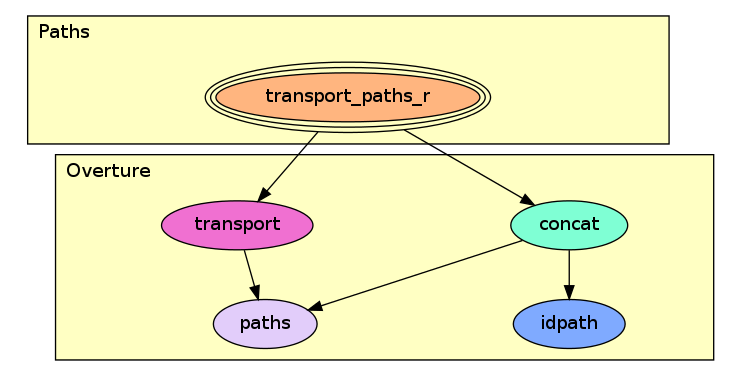
\includegraphics[scale=.35]{graphpaths.png}
\caption{\scriptsize{\emph{Dependency graph for the definition of \texttt{transport\_paths\_r} included in the \texttt{Paths} library of HoTT.}}}\label{fig:dgraph2}
\end{figure}


Coq also supports the visualisation of the proof-tree during an interactive proof development using the Prooftree tool~\cite{prooftree}. This tool was aimed to visualise the different subgoals that arise during the development of a proof, see Figure~\ref{fig:prooftree}. ML4PG automaton representation of proofs (cf. Figure~\ref{fig:automata}) not only shows the applied tactics, but also the generated-subgoals in each step, and compare the proof flow of the current proof with the steps followed in other theorems. 

\begin{figure}
\centering
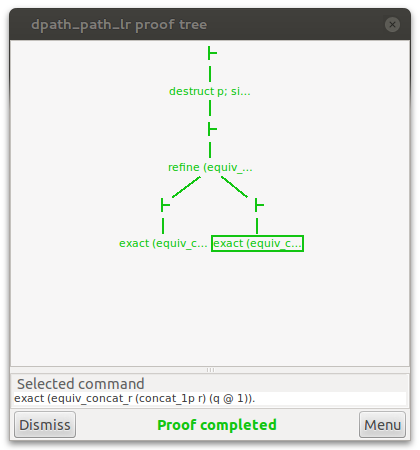
\includegraphics[scale=.5]{prooftree.png}
\caption{\scriptsize{\emph{Proof tree for the theorem \texttt{dpath\_path\_lr} included in the \texttt{Paths} library of HoTT.}}}\label{fig:prooftree}
\end{figure}

Finally, the tool presented in~\cite{GNR14} can infer models from Coq developments. Those models are represented as automata that are latter used to generate proof attempts. Since the models were designed with the aim of automatically generate proofs, they are not human-readable. 
ML4PG's graphical representation of automata is simpler than the work presented in~\cite{GNR14}.  





